\chapter{Methodology}
\label{chap:3}

\section{Introduction} 

Dark matter, an invisible material that comprises about 27 percent of the universe, has long been a focus of astrophysics research. It would be one of the important constituents of the universe, yet hitherto has escaped conventional detection. Dark matter is fundamental to explaining how galaxies form and the gravitational forces at work in the cosmos. The methods of study of the dark matter are based on complex analysis using supercomputers, data obtained from astronomical observations and advanced mathematical models. They are frequently based on Machine Learning (ML) algorithms aimed at helping to interpret complicated data and perform predictions of the behavior/properties of dark matter.



\section{Apparatus and Procedure for Computer Data Collection and Simulation}

For dark matter studies, data are usually obtained with sophisticated observatories and telescopes which combine multiple observations including galaxy clusters and gravitational lenses. Computer simulations are then employed to follow dark matter’s potential impact on these cosmic features. Such simulations provide a way to simulate under controlled conditions and powerfully test hypotheses about the nature of dark matter, in particular predicting how it interacts with visible matter and gravitational fields.

\section{Data Pre-processing}

Observational data obtained from different astronomical facilities may be noisy, not complete or in formats difficult to analyze. This data needs to be cleaned and processed before it is ready for analysis. Basics like cleaning noises, filling NAs, normalizing data are the most important step to avoid any distorted learning from ML models.
\section{Multivariate Analysis}
\begin{figure}[H]
    \centering
    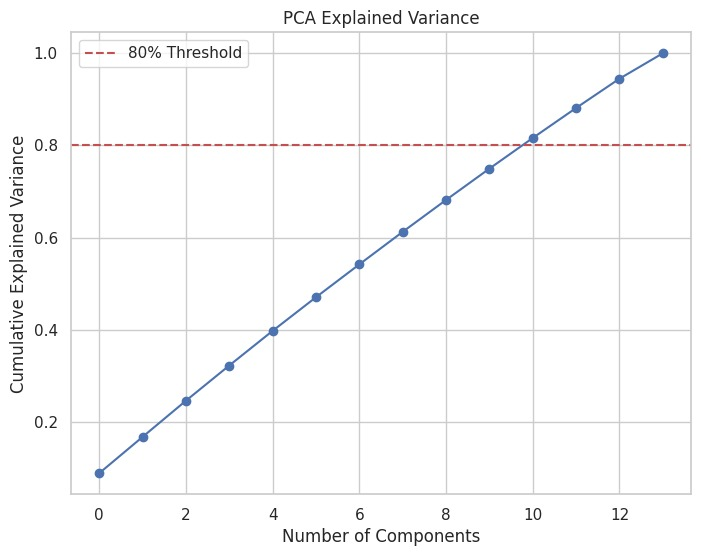
\includegraphics[width=1\linewidth]{Chap3/pca_explained_variance.jpeg}
    \caption{PCA Explained Variance}
    \label{fig:placeholder}
\end{figure}

This figure gives the Scree Plot, i.e. a cumulative variance plot of PCs from a PCA over a dataset.

\begin{itemize}
    \item The horizontal x-axis is the number of components, and the vertical y-axis is the cumulative explained variance.

    \item The figure reveals a continuous growth of the variance for higher and higher parts, that leads to a value close to 1.

    \item Above the plot a visible red line can be seen at 80\% which corresponds to what amount of variance (80\%) is represented by the respective principal components.
\end{itemize}
\begin{figure}[H]
    \centering
    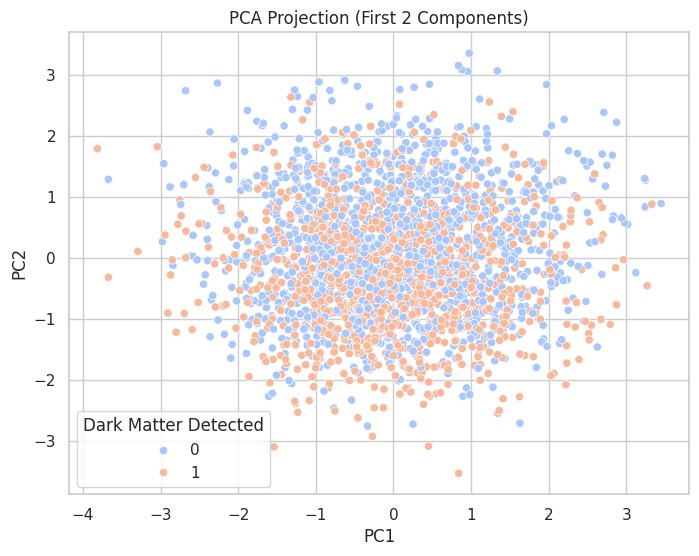
\includegraphics[width=1\linewidth]{Chap3/pca_projection.jpeg}
    \caption{First 2 component Projection}
    \label{fig:placeholder}
\end{figure}

This is a scatter plot that illustrates the data projected on to the first two principal components(PC1 and PC2) from PCA.

\begin{itemize}
    \item The x axis represents PC1 and the y axis denotes PC2.

    \item The data points are shaded whether or not dark matter is present, with blue representing "0" (no DM detection) and orange representing "1" (DM detection).

    \item This visualization allows checking how the first two components separate the two classes.
\end{itemize}
 
\section{Feature Selection and Engineering}

Feature selection and feature engineering are both crucial for enhancing the performance of ML models in dark matter paradise. The trained model is then tested with selected features (gravitational lensing data, galaxy cluster properties etc.). Time and space transformation of the raw data can produce new variables to improve model results (eg, derivation of composite indices from different observation measures).

\section{Machine Learning Models Used}

In the field of dark matter, there are few different ML techniques used and supervised methods play an important role. These algorithms are trained on annotated samples to learn patterns and predict data. Popular techniques are decision trees, random forests, and neural networks. Machine learning (ML) models can assist with categorizing dark matter-related events, make predictions about its distribution through the universe and also simulate potential interactions between this stuff and other forces in the cosmos.

\section{Advantages of Using Machine Learning}

The ML brings the following benefits to dark matter study. ML models have the advantage of handling massive and complicated datasets, becoming better at predicting patterns from the apparently concealed information and enhance predictability of simulations. They also make a complete framework that can fully automatize the search for the dark matter signatures in observational data from which we obtain faster and less demanding search than by hand.

\section{Supervised Algorithms}

Supervised learning techniques, such as SVMs, logistic regression and neural network are often used to classify some of the properties associated with the dark matter. They are trained with labeled data (example of which we already know their outcomes) in order to learn the true connections between features and target values. The information they learn in this training is then used by the algorithms to enable them to predict how the system will react when given new, unseen data, and there you have it: A glimpse into some of dark matter’s elusive behaviors.
 
 


\section{System Implementation}
\subsection{Performance Indicators}


Performance measures are critical to assess and compare the performance of machine learning model. They give the intuition about how well a model is doing on the problem you want it to solve. Performance measures comprise the accuracy, precision recall (sensitivity), F1 score, and model efficiency. And each of these metrics has a specific role to play in capturing some feature of the model behavior. These statistics are indispensable for both evaluating and refining the model to achieve optimal performance in a particular task.


\subsection{Analysis of the Confusion Matrix} 
The confusion matrix is a widely used technique to evaluate the classification models. It does gives a good in-depth breakdown of the true positives, true negates, false positives, and falls negatives. We can use the confusion matrix to compute a lot of performance metrics like accuracy, precision, recall and F1 score. The confusion matrix is a visual representation of how well the model is doing for classifying data to different classes, it makes it easy to identify where the model might be going wrong. This matrix is fundamental to interpret the strengths and weaknesses of the model on different category predictions.

 

\begin{table}[h!]
\centering
\begin{tabular}{|c|c|c|}
\hline
                & Predicted Positive & Predicted Negative \\ \hline
Actual Positive & True Positive (TP) & False Negative (FN) \\ \hline
Actual Negative & False Positive (FP) & True Negative (TN) \\ \hline
\end{tabular}
\caption{Confusion Matrix}
\label{tab:confusion_matrix}
\end{table}


\subsection{Accuracy}

Accuracy is the easiest and most straightforward performance measure. The ratio of correct predictions (True Positive + True Negative) to the total number of predictions made. On the other hand, accuracy provides a fast—but incomplete—picture of how a model is performing and can be misleading if the dataset is unbalanced. For example, in a very imbalanced dataset the model which always predicts the majority class can have high accuracy yet still suck at finding the minority class. Thus, accuracy should not be viewed in isolation but studied along with other metrics to have an integrated view of a model's performance.

Where:

TP = True Positives

TN = True Negatives

FP = False Positives

FN = False Negatives
 \begin{equation}
\text{Accuracy} = \frac{TP + TN}{TP + TN + FP + FN}
\end{equation}

 

\subsection{Precision}
Precision, just as a reminder that it’s sometimes called positive predictive value as well, is the rate at which our classifier generates true positives. It addresses the question: of all positive predictions by the model, how many were positive? Accuracy is crucial when false positives are cost-prohibitive or unjustifiable. If, say, a medical diagnosis model misclassifies healthy people as sick, it could prompt unnecessary tests or treatments. High precision indicates high trust in positive predictions.


\begin{equation}
\text{Precision} = \frac{TP}{TP + FP}
\end{equation}



\subsection{Recall or Sensitivity}

Recall, or sensitivity, indicates the percentage of true positive instances that were accurately predicted by the model. e. true positives) the model was able to identify? Recall is particularly significant in the presence of severe costs associated with missing positive cases. For instance, in a fraud detection system not detecting fraudulent transactions (false negatives) might result in large losses. High recall means the model is catching as many of the true positive results as possible.


\begin{equation}
\text{Recall} = \frac{TP}{TP + FN}
\end{equation}

\subsection{\textbf{F1 Score}}
The F1-score is the harmonic mean of precision and recall. It is a compromise between precision and recall that weights the two equally. F1 score is especially helpful when you have an uneven class distribution and moreover false positive and false negatives are of significant cost. Unlike accuracy which can be affected by a class imbalance, F1 score takes into account both the ability to identify positive cases (recall) and whether the predictions are correct or not (precision). A high F1 score means a model with good precision and recall.
 

\begin{equation}
\text{F1 Score} = 2 \times \frac{\text{Precision} \times \text{Recall}}{\text{Precision} + \text{Recall}}
\end{equation}




\subsection{Model Efficiency}
Model area computation efficiency indicates how efficiently a machine learning model can be computed in terms of resources (time, memory, and processing power) needed during both training and inference. Although precision or other performance measures are crucial, model efficiency is equally important, in particular when running in real-time or when processing large amounts of data. Machines can predict faster and take up less computational power. The overall models should be used for deployment if the amount of data is large enough to warrant an overall infrastructure that includes smaller size nodes. Trade-off between model accuracy and efficiency makes the model not only good in performance, but also feasible in the engineering application.